\section{Theorie}
\subsection{Newtonsche und Lagrangsche Mechanik}
In folgenden soll die Herleitung der bewengungsgleichung des Doppelpendels mit Hilfe des Lagrange-Formalismus der klassischen Mechanik beschrieben werden. \\
Die Bewegungsgleichung eines [mechanischen Systems] Massepunktes und deren Lösung $\vec{x}(t)$ lassen sich nach Newton aus der Summe aller an der Masse greifenden Kräfte bestimmen, also es gilt \begin{equation}
\vv{\ddot{x}}=\frac{1}{m}\sum \vv{F}
\end{equation}
In der Praxis - so auch beim Doppelpendel - stellt es sich als äußerst schwierig dar, alle am Massepunkt wirkenden Kräfte zu identifizieren sowie mathematisch zu beschreiben. Als eine Art Verallgemeinerung der newtonschen Mechanik lässt sich aus ihr [mit Hilfe des hamiltonischen Prinzips] der sogenannte Lagrange-Formalismus herleiten. Hier sind die gesuchte Funktionen die Lösungen der Lagrange-Gleichungen
\begin{equation}
\frac{d}{dt}\frac{\partial L}{\partial\dot{x_i}}-\frac{\partial L}{x_i} = 0
\end{equation}
mit der Lagrangefunktion  $ L=E_{kin} - V $ . Hierbei sind $E_{kin}$ die kinetische Energie und v das auf den Massepunkt wirkende Potential. Ein weiterer Vorteil dieses Formalismus besteht darin, dass die Langrangegleichungen unter Koordinatenfunktionen invariant bleiben, es gilt also:
\begin{equation}
\frac{d}{dt}\frac{\partial L}{\partial\dot{q_i}}-\frac{\partial L}{q_i} = 0
\end{equation}
Hier sind $q_i$ die verallgemeinerten Koordinaten, die so gewählt werden, damit alle geometrischen Einschränkungen, denen das mechanische System unterworfen ist (sog. Zwangsbedingungen) berücksichtigt werden und die Anzahl der Freiheitsgrade berücksichtigt werden. Für jeden Freiheitsgrad muss nun eine Lagrangegleichung aufgestellt werden.
\subsection{Das Doppelpendel}
Im Ursprungspunkt des Koordinatensystems wird ein Pendel, bestehend aus einem Stab mit fester Länge $l_1$ und einer Masse m an dessem Ende befestigt. Das Pendel soll sich nur in der x-z Ebene bewegen können, Am Massenpunkt befindet sich nun ein zweites Pendel mit Stab der Länge $l_2 \rightarrow l_1$ [und mit gleicher Masse], welchess sich ebenso nur in der x-z-Ebene bewegenn soll. \\
Der erste Schritt besteht nun darin, eine Beschreibung der Ortsvektoren der beiden Massenpunkte zu finden[, die alle Zwangsbedingungen berücksichtigen]. Die Masse $ m_1 $ ist wie erwähnt Bestandteil eines normalen Pendels in der Ebene. Daraus folgt für $ \vv{x_1} $
\begin{equation}
\vv{x_1}= l_1*\begin{pmatrix}
\sin \varphi_1 \\ -\cos \varphi_1
\end{pmatrix}
\end{equation}
[Hierbei ist $ l_1 $ die Länge des ersten Pendels und $ \varphi_2 $ dessen Auslenkung aus der Ruhelage.]
Die Masse $ m_2 $ ist ebenso Teil eines Pendels, das an $m_1$ aufgehängt ist, also müssen die Orte der Massen addiert werden. Für den Vektor $\vv{x_2}$ folgt:
\begin{equation}
\vv{x_2}= \vv{x_1} + l_2 * \begin{pmatrix}
\sin \varphi_2 \\ -\cos \varphi_2
\end{pmatrix}
= \begin{pmatrix}
l_1 * \sin \varphi_1 + l_2 * \sin \varphi_2 \\ - l_1 * \cos \varphi_1 - l_2 * \cos \varphi_2
\end{pmatrix}
\end{equation}


Zur Bestimmung von $E_{kin,i} = \frac{m_i}{2} * \dot{\vv{x_i}}^2$  müssen noch die Ableitungen der Ortsvektoren gebildet werden:
\begin{equation}
\dot{\vv{x_1}} = l_1*\dot{\varphi_1}*\begin{pmatrix}
\cos \varphi_1 \\ \sin \varphi_1
\end{pmatrix}
\end{equation}
und:
\begin{equation}
\dot{\vv{x_2}} = \dot{\vv{x_1}} + l_2 * \dot{\varphi_2} * \begin{pmatrix}
\cos \varphi_2 \\ \sin \varphi_2
\end{pmatrix} 
\end{equation}
Für die kinetische Energie ergibt sich:
\begin{equation}
E_{kin} = E_{kin,1} + E_{kin,2} = \frac{m_1}{2} * l_1^2 * \dot{\varphi_1}^2 +
\frac{m_2}{2} * (l_1^2 * \dot{\varphi_1}^2 + l_2^2 * \dot{\varphi_2}^2 + 2 * l_1 * l_2 * \dot{\varphi_1} * \dot{\varphi_2} * \cos (\varphi_1 - \varphi_2))
\end{equation}
Das auf das Doppelpendel wirkende Potential $ V_i = m_i * g * h_i $ ist:
\begin{equation}
V = V_1 + V_2 = m_1 * g * (-l_1 * \cos \varphi_1) + m_2 * g * (-l_1 * \cos \varphi_1 - l_2 * \cos \varphi_2)
\end{equation}
Die Aufstellung der Lagrange-Gleichung erfolgt nun in mehreren Schritten. Zuerst für $ \varphi_1$ :
\begin{equation}
\frac{\partial (E_{kin} - V)}{\partial\dot{\varphi_1}} = (m_1 + m_2) * l_1^2 *\dot{\varphi_1} + m_2 * (l_1 * l_2 * \dot{\varphi_2} * \cos (\varphi_1 - \varphi_2)) 
\end{equation}
\begin{equation}
\frac{\partial (E_{kin} - V}{\partial \varphi_1}} = -m_2 l_1 l_2 \dot{\varphi_1} \dot{\varphi_2} \sin (\varphi_1 - \varphi_2) - (m_1 + m_2) g l_1 \sin \varphi_1
\end{equation}
und nun für $ \varphi_2 $ :
\begin{equation}
\frac{\partial (E_{kin} - V}{\partial }dot{\varphi_2}}} = m_2 l_1 l_2 \dot{\varphi_1} \dot{\varphi_2} \sin (\varphi_1 - \varphi_2) - m_2 g l_2 \sin \varphi_2
\end{equation}
\begin{equation}

\frac{\partial (E_{kin} - V}{\partial \varphi_2}} = m_2 l_2^2 \dot{\varphi_1} \dot{\varphi_2} + m_2 l_1 l_2 \dot{\varphi_1} \cos (\varphi_1 - \varphi_2)
\end{equation}
Setzt man diese Terme in (3) ein, erhält man die Bewegungsgleichungen des Systems:
\begin{equation}
\frac{d}{dt}\frac{\partial L}{\partial\dot{q_i}}-\frac{\partial L}{q_i} = (m_1 + m_2) _1^2^\ddot{\varphi_1} + m_2 l_1 l_2 \ddot{\varphi_2} \cos (\varphi_1 - \varphi_2) + m_2 l_1 l_2 \dot{\varphi_2}^2 \sin (\varphi_1 - \varphi_2) + (m_1 + m_2) g l_1 \ sin \varphi_1 = 0
\end{equation}
\begin{equation}
\frac{d}{dt}\frac{\partial L}{\partial\dot{q_i}}-\frac{\partial L}{q_i} = m_2 l_2^2 \ddot{\varphi_2} + m_2 l_1 l_2 (\ddot{\varphi_1} \cos (\varphi_1 - \varphi_2) - \dot{\varphi_1}^2 \sin (\varphi_1 - \varphi_2)) + m_2 g l_2 \sin \phi_2 = 0
\end{equation}


\subsection{Simulation des Doppelpendels}
Mithilfe eines Python-Skripts wurden die in der Theorie hergeleiteten Differenzialgleichungen für das Doppelpendel numerisch gelöst. Dafür wurden die Differenzialgleichungen zunächst nach $ \ddot{\phi_1} $ und $\ddot{\phi_2} $ aufgelöst: 

\begin{equation}
(m_1 + m_2) l_1 \ddot{\phi_1}  + m_2 l_2 \ddot{\phi_2} \cos{(\phi_1 - \phi_2)} + m_2 l_2 \dot{\phi_2}^{2} \sin{(\phi_1 - \phi_2)} + g (m_1 + m_2) \sin{\phi_1} = 0
\end{equation} 
und
\begin{equation}
m_2 l_2 \ddot{\phi_2} + m_2 l_1 \ddot{\phi_1} \cos{(\phi_1 - \phi_2)} - m_2 l_1 \dot{\phi_1}^{2} \sin{(\phi_1 - \phi_2)} + g m_2 \sin{\phi_2} = 0
\end{equation}
. 

Um die Gleichungen mittels eines Standardverfahrens numerisch lösen zu können, muss das Gleichungssystem auf die Form $ \dot{Y} = f(Y) $ gebracht werden. Zunächst werden die obigen Gleichungen nach $ \ddot{\phi_1} $ und $ \ddot{\phi_2} $ aufgelöst. Es ergibt sich unter Beachtung der folgenden abkürzenden Notation: 
$ (m_1 + m_2) =: M; \phi_1 - \phi_2 =: \Delta \phi $
\begin{equation}
\ddot{\phi_1} = \frac{-m_2 l_2 \dot{\phi_2}^{2} \sin{\Delta \phi} - g M \sin{\phi_1} - m_2 l_1 \dot{\phi_1}^{2} \sin{\Delta \phi} \cos{\Delta \phi} + g m_2 \sin{\phi_2}\cos{\Delta  \phi}}{M l_1 - m_2 l_1 \cos^{2}{\Delta \phi}}
\end{equation}
und
\begin{equation} 
\ddot{\phi_1} = \frac{-m_2 l_2 \dot{\phi_2}^{2} \sin{\Delta \phi} \cos{\Delta \phi} - g M \sin{\phi_1} \cos{\Delta \phi} - M l_1 \dot{\phi_1}^{2} \sin{\Delta \phi} + g M \sin{\phi_2}}{m_2 l_2 \cos^{2}{\Delta \phi} - M l_2}
\end{equation}

Dieses Differenzialgleichungssystem erster Ordnung kann nun mit Hilfe elementarer Algorithmen gelöst werden. Hier wurde das expliztite Euler-Verfahren verwendet (\ref{}). Es wurde also ein Vektor $$ \vec{\phi} = (
\phi_1, \dot{\phi_1}, \phi_2 , \dot{\phi_2})^{T} $$ 
 definiert, für den sich ergibt: 
\begin{equation}
\dot{\vec{\phi}} = (\dot{\phi_1}, \ddot{\phi_1}, \dot{\phi_2}, \ddot{\phi_2})^{T}
\end{equation}
, wobei für $ \ddot{\phi_1} $ und $ \ddot{\phi_2} $ obige Gleichungen eingesetzt werden. 
Dann wird eine schrittweise Iteration durchgeführt, der Quelltext für das verwendete Python-Skript findet sich im Anhang. 

\subsection{Reibung}
Bei dem hier behandelten Doppelpendel treten im Wesentlichen Luftreibung und Reibung in der Lagerung der zueinander beweglichen Bauteile, also den Kugellagern. Darüber hinaus tritt weiterer Energieverlust auf, indem die Aufhängung des Pendels vom Pendel selbst zu Schwingungen angeregt wird und so ein Energieübertrag stattfindet. 

\subsubsection{Luftreibung}
Für die Luftreibungskraft, die auf einen laminar umströmten Gegenstand wirkt, gilt die in guter Näherung gültige Formel
\begin{equation}
F_R = v^2 \cdot \frac{\rho}{2} \cdot A_S \cdot c_W
\end{equation}, 
wobei $ F_R $ die Luftreibungskraft, $ v $ die Geschwindigkeit der umströmenden Luft, $ \rho $ deren Dichte, $ A_S $ die Fläche der Projektion des Gegenstands in Stömungsrichtung und $ c_W $ ein von der Form des Gegenstands bestimmter, dimensionsloser Koeffizient ist. 


\subsubsection{Reibung in den Kugellagern}
Für die Reibung in den Kugellagern kann das Modell der Rollreibung verwendet werden. Demnach ergibt sich für die Reibungskraft $ F_R $:
\begin{equation}
F_R = c_R \cdot F_N
\end{equation}, 
wobei $ c_R $ ein die verwendeten Materialien und deren Form charakterisierender Parameter ist und $ F_N $ der Betrag der Normalkraft, also die senkrecht zur Rollrichtung wirkende Kraft. 

\subsubsection{Energieübertrag auf die Aufhängung}

Die Betrachtung dieser Art von Energieverlust ist schwierig. Zwar könnte er mit dem Modell zweier gekoppelter schwingfähiger Systeme, bei dem das zweite eine große Dämpfung aufweist, angenähert werden. Allerdings müsste hierfür wieder der Lagrange-Formalismus herangezogen werden, wobei zusätzlich noch Reibungsterme berücksichtigt werden müssten. 



\subsubsection{Phasenraumkurven und Attraktoren}
Der Phasenraum eines Systems ist der Raum, dessen Koordinaten die Zustandsgrößen des Systems sind. (z.B. $x, \dot{x}$) Eine Kurve $X(t) = (x(t), \dot{x}(t))^T$ im Phasenraum heißt \textbf{Trajektorie} und beschreibt die zeitliche Entwicklung des Systems. Zeitlich konstante Punkte im Phasenraum, an denen die Geschwindigkeit des Massepunkts $\dot{X}(t) = 0$  ist, nennt man \textbf{Fixpunkte}. Kurven im Phasenraum können sich nur in Fixpunkten schneiden, da die zeitliche Entwicklung des Systems eindeutig durch die Anfangsbedingungen vorgegeben ist. Da in Fixpunkten mehrere (im Allgemeinen sogar unendlich viele) Trajektorien zusammenlaufen können, nennt man solche Fixpunkte auch \textbf{Attraktoren}. In nichtlinearen Systemen können Attraktoren auch andere Formen (z.B. Flächen oder Kurven) annehmen, sind dann aber keine Fixpunkte mehr.
\\
Phasenraumkurven sind ein praktisches Mittel, um das Verhalten von (chaotischen) Systemen zu zeigen, wie man in den folgenden Beispielen sehen kann.

\begin{figure}
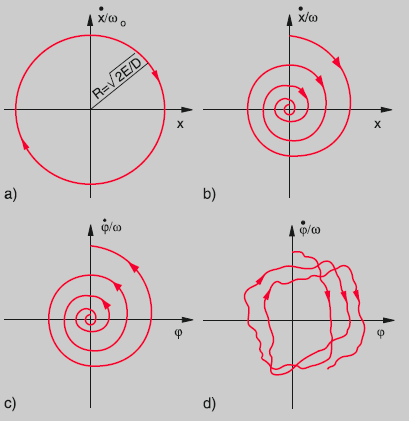
\includegraphics[width=1.0\textwidth]{phasenraum1.png}
\caption{Phasenraumkurven von: \\a) ungedämpfter harmonischer Oszillator \\b) gedämpfter harmonischer Oszillator \\c) harmonischer Oszillator mit negativer Dämpfung \\d) nichtlinearer angeregter Oszillator im chaotischen Bereich \\Herleitung siehe Demtröder \textbf{HIER REFERENZ ZUM LITERATURVERZEICHNIS EINFÜGEN}}
\end{figure}

\begin{figure}
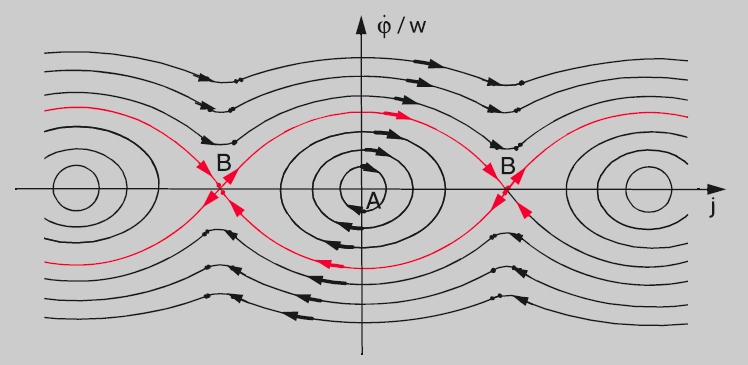
\includegraphics[width=1.0\textwidth]{phasenraum2.png}
\caption{Phasenraumkurven eines ungedämpften Fadenpendels. Der Punkt A ist Attraktor für alle Winkel $|\phi|<\pi$. Die rote Kurve stellt eine 'Grenzkurve' zwischen stabilen und instabilen Lösungen dar. Die Punkte B ($|\phi|=180\deg, \dot{\phi}=0$) sind instabile Fixpunkte, eine minimale Änderung des Winkels wird eine stabile Pendelbewegung erzeugen, eine minimale Änderung der Winkelgeschwindigkeit wird eine Rotationsbewegung erzeugen, bei der der Winkel unbegrenzt ansteigt.}
Herleitung siehe Demtröder \textbf{HIER REFERENZ ZUM LITERATURVERZEICHNIS EINFÜGEN}
\end{figure}
